\section{Algorithms}
\label{sec:algorithms}

In the last section, we presented how \conveinsum represents general multi-linear operations in (compact) neural networks.
In this section, we develop a suite of algorithms to implement the \conveinsum function efficiently. We organize this section as follows: 
\textbf{(1)} In \Cref{sub:algorithms-atomic}, we develop an algorithm to reduce a \conveinsum function with two inputs to a collection  of atomic \pytorch operations, which allows us to reuse GPU-optimized functions in \pytorch to complete the computation. 
\textbf{(2)} In \Cref{sub:algorithms-sequencer}, we derive an optimal sequencer which automatically decomposes a \conveinsum function with an arbitrary number of inputs into a sequence of \conveinsum functions with two inputs;
\textbf{(3)} In \Cref{sub:algorithms-checkpointing}, we utilize a {\em checkpointing} technique to further reduce the memory overhead of our implementation.

\subsection{Atomic Operations}
\label{sub:algorithms-atomic}

We can represent a \conveinsum function with two inputs via GPU-optimized \pytorch functions, specifically \einsum and \convNd (e.g., \convOne, \convTwo).
%If there is no letter for convolution, we can simply use \einsum function.
In particular, we will show that any \conveinsum function with convolution can be realized via \convNd. To understand why such a transformation is possible, we first analyze the \conveinsum string for the \convOne function:
\begin{lstlisting}
Y = conv_einsum("bsh,tsh->bth|h", X, W)
\end{lstlisting}
\vspace{-1em}
where \textsf{"t"} stands for the output channel, \textsf{"s"} the input channel, \textsf{"h"} the length of features/filters, and \textsf{"b"} the batch size. Now, we can categorize these letters in terms of primitive operations.
\textbf{(1)} The letter \textsf{"h"} is a convolution, 
appearing in both inputs and the output;
\textbf{(2)} The letter \textsf{"s"} is a contraction, 
appearing in both inputs but not the output;
\textbf{(3a)} The letter \textsf{"t"} is an outer product,
appearing in the first input and the output;
\textbf{(3b)} The letter \textsf{"b"} is another outer product,
appearing in the second input and the output.

The \convOne function covers almost all mixtures of compound multi-linear operations in which each operation type appears at most once, which we refer to as an \textit{atomic operation}. However we have two cases which are not covered:
\textbf{(4)} A batch product that appears in both inputs and the output; and
\textbf{(5)} A self-contraction that appears in only one input.
Fortunately, these two edge cases can be easily addressed.
For \textbf{(4)}, the function \convOne supports a group-convolution option, which effectively extends to:
\begin{lstlisting}
Y = conv_einsum("gtsh,bgsh->bgth|h", X, W)
\end{lstlisting}
\vspace{-1em}
where \textsf{"g"} stands for the filter group. In terms of tensor operations, it is a batch product, which appears in both inputs and the output. For \textbf{(5)}, such a letter can be eliminated by summing over the corresponding index in pre-processing.

In summary, \textbf{(1)-(5)} cover all possible types of tensor operations; the function \convOne covers \textbf{(1)-(4)} and \textbf{(5)} can be addressed via a pre-processing. Thus, paired with index-swapping operations, \convOne can realize any \conveinsum string where each operation type appears only once.

% Discussion of multiple letters
\textbf{Multiple letters with the same operation type.} 
Now we will address the scenario where there are multiple letters with the same operation type. For example, if there are two different letters in a \conveinsum string designated for convolution, we can use \convTwo instead of \convOne. Notice that \convTwo realizes a \conveinsum such as:
\begin{lstlisting}
Y = conv_einsum("gtshw,bgshw->bgthw|h,w", X, W)
\end{lstlisting}
\vspace{-1em}
where \textsf{"g"}  stands for the filter group and \textsf{"h"}/\textsf{"w"}  represent height/width of the filters/features respectively. In principle, we can use a \convNd function to compute a \conveinsum function with $N$ letters for convolution (though \convNd for $N \geq 4$ requires custom implementation).

For non-convolution letters, all letters with the same type can be merged into one letter in the preprocessing (i.e., the corresponding modes are reshaped into one compound mode), and the letter is converted back to multiple letters in the post-processing step (i.e., the compound mode is reshaped into its corresponding modes).

% figure for optimal sequencer
\begin{figure*}[!htbp]
\begin{minipage}[b]{.38\linewidth}
\centering
\begin{lstlisting}
A=np.random.rand(4,7,9)
B=np.random.rand(10,5)
C=np.random.rand(5,4,2)
D=np.random.rand(6,8,9,2)
path_info = conv_einsum.contract_path("ijk,jl,lmq, njpq->ijknp|j", A, B, C,D)
print(path_info[1])
\end{lstlisting}
\subcaption{\textbf{Tensor sequence generation.} A tensor sequence over a collection of tensors $\tensor{A}, \tensor{B}, \tensor{C}$, and $\tensor{D}$, involving contractions, convolutions, and batch products is analyzed. We store and print the optimal sequence of paths, which is stored in a string array \texttt{path\_info}.}
\label{fig:cvoutput-a}
\end{minipage}%
\hfill
\begin{minipage}[b]{.6\linewidth}
\centering
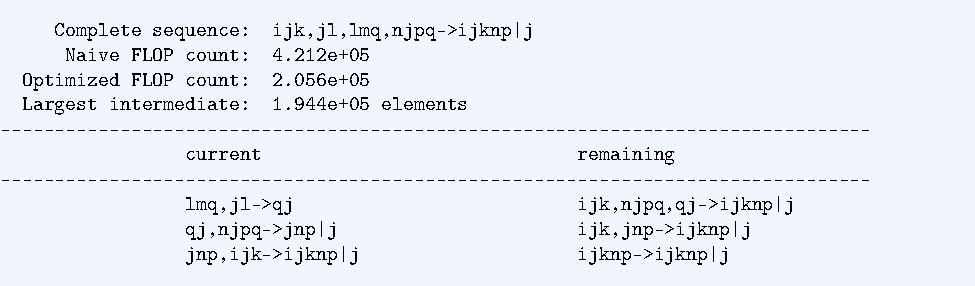
\includegraphics[width=0.98\textwidth]{\fighome/cvoutputfinal.pdf}
\subcaption{\textbf{An optimal sequence of paths.} The code, leveraging \opteinsum with our added support for convolutions, displays the optimal sequence of paths for the \conveinsum string submitted in Figure \ref{fig:cvoutput-a}. We are also presented with information about the naive left-to-right cost vs the cost of taking the suggested path, along with the size/cost of the largest intermediate.}
\label{fig:cvoutput-b}
\end{minipage}
\vspace{-1em}
\caption{\textbf{\conveinsum sample code.} The figure depicts the generation via \numpy of a set of tensors coalesced into one tensor sequence. The sequence is represented as a string and submitted to optimal sequencer of \conveinsum for path analysis. The output of the analysis is presented in Figure \ref{fig:cvoutput-b}.}\label{fig:cvoutput}
\end{figure*}





\begin{figure*}[!ht]
\begin{centering}
 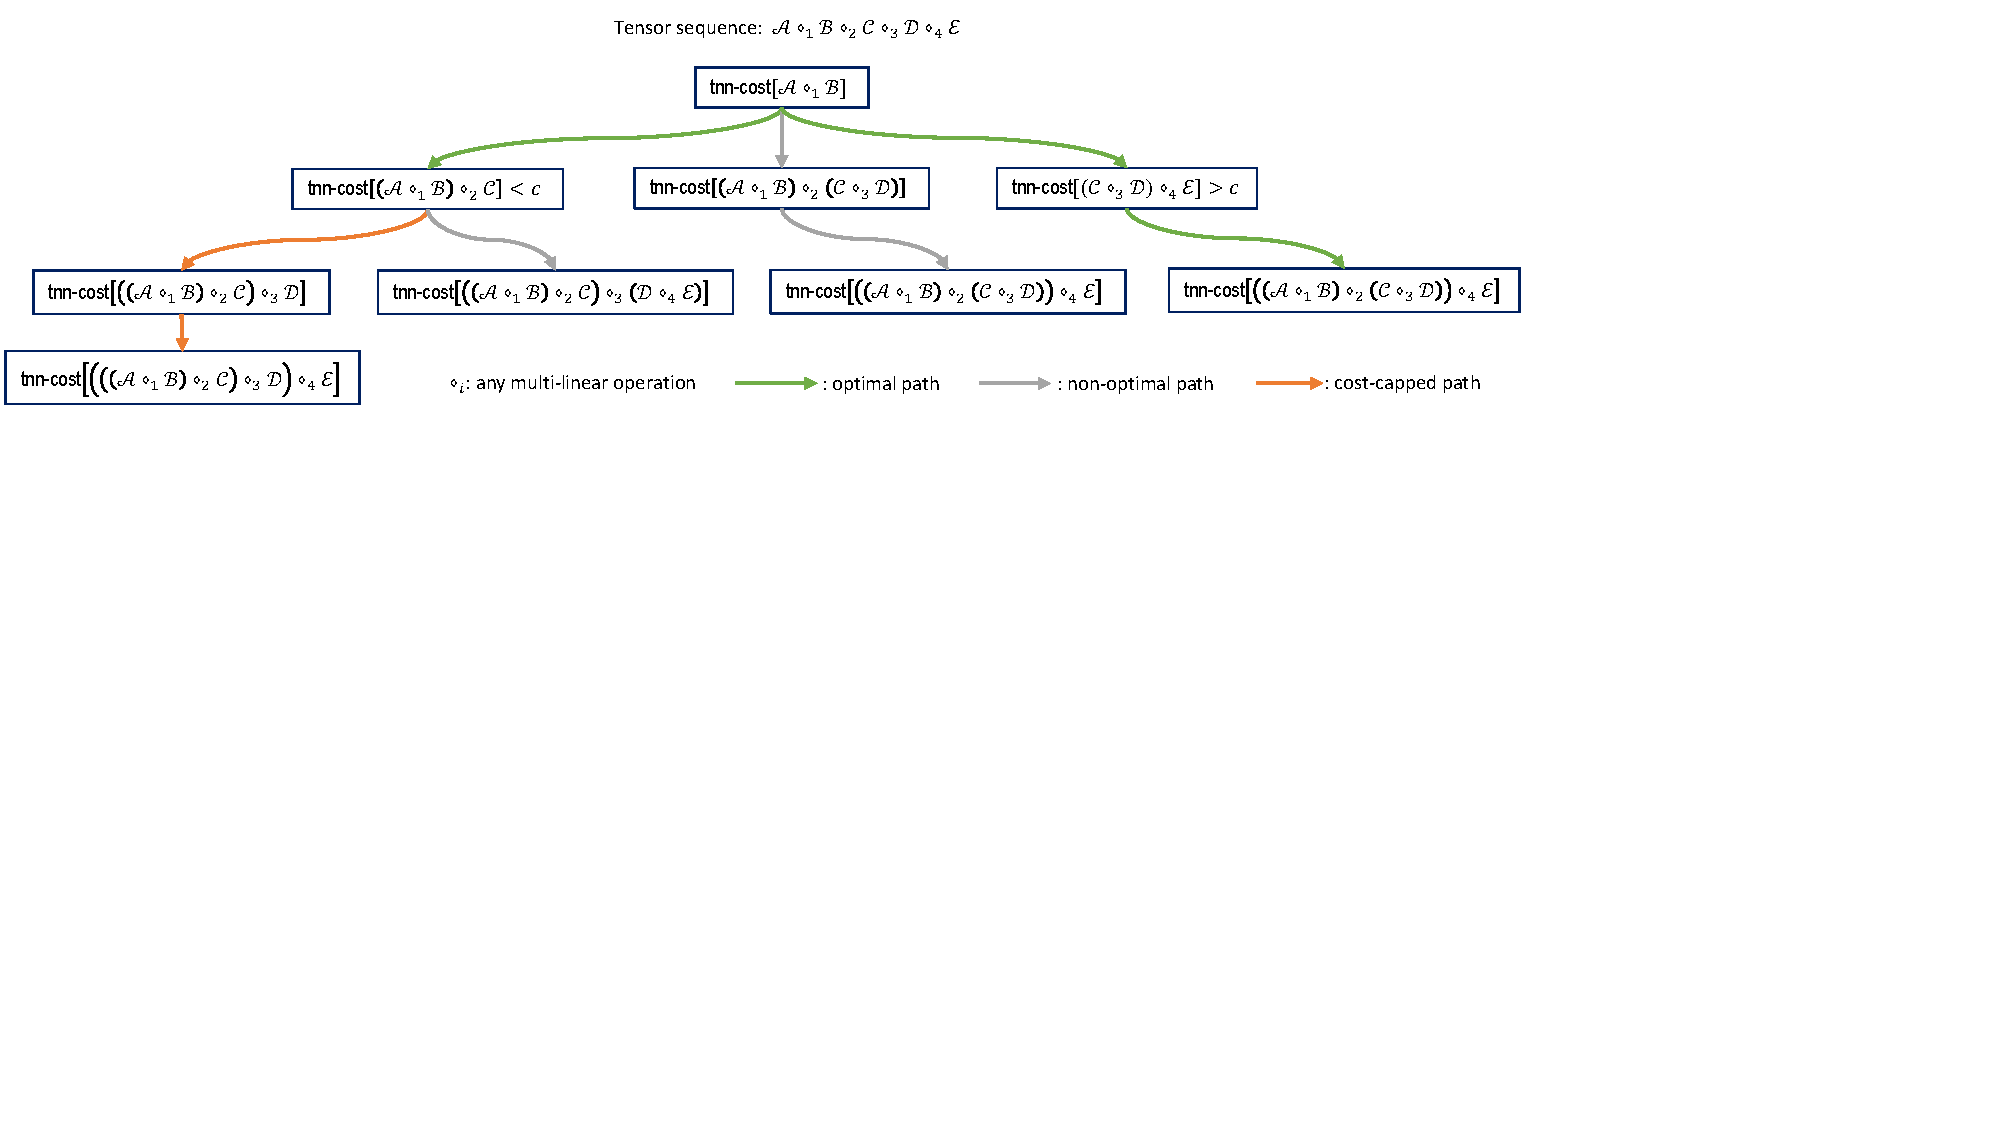
\includegraphics[width=0.9\textwidth]{\fighome/optimal-sequencer.pdf}
 \vspace{-0.5em}
 \caption{\textbf{Optimal sequencer example}. In this figure, \conveinsum deploys the optimal sequencer to analyze the path tree of an abstract, well-defined tensor sequence $\tensor{A} \circ_1 \tensor{B} \circ_2 \tensor{C} \circ_3 \tensor{D} \circ_4 \tensor{E}$, where $\circ_i$ for $1\leq i \leq 4$ is any collection of multi-linear operations, including convolutions, batch products, contractions, and outer products. The tree traversal strategy is a fusion of \netcon and our \textsf{tnn-cost} API. The green path indicates a potentially viable optimal path, whereas the red path indicates a path which satisfies the cost cap $c$ at each node. While the red path satisfies the cost cap, it may result in more FLOPs overall compared to the complete green path.
 \vspace{-1em}}
 \label{fig:opt-seq}
\end{centering}
\end{figure*}

\subsection{Optimal Sequencer}
\label{sub:algorithms-sequencer}

Our \conveinsum leverages APIs in the existing open-source \opteinsum library for \numpy \citep{daniel2018opt}. The \opteinsum library can handle determining the FLOPs-optimal evaluation order of tensor networks involving contractions, outer products, and batch products. 
Our \conveinsum introduces convolution handling to \opteinsum. Due to the code complexity of our convolutional-functionality and the core APIs of \opteinsum, we instead present a high-level overview of the basis of \conveinsum. 

The \opteinsum library relies on the well-known \netcon \citep{pfeifer2014faster} algorithm for determining an optimal order of evaluations. \netcon was designed to handle operation sequences in tensor networks. For example, for $\tensor{A} \in \R^{I \times J \times K}, \tensor{B} \in \R^{J \times L}, \tensor{C} \in \R^{L \times M}$, one might be interested in the optimal order of evaluation of the tensor
\begingroup
\abovedisplayskip=5pt
\belowdisplayskip=5pt
\begin{equation}
\label{eq:net-consequence}
\tensor{T} = \sum_{l = 1}^{L} \sum_{j = 1}^{J}
\tensorSub{A}{\slice, j, \slice} \otimes \tensorSub{B}{j,l} \otimes \tensorSub{C}{l, \slice}.
\end{equation}
\endgroup
Let us momentarily suppress the index and summation notation of \Cref{eq:net-consequence}, i.e., let $(AB) \triangleq \sum_{j=0}^{J-1}\mathcal{A}_{:,j,:}\mathcal{B}_{j,l}$, $(BC)\triangleq \sum_{l=0}^{L-1}\mathcal{B}_{j,l}\mathcal{C}_{l,:}$. The possible paths we may take to arrive at $\tensor{T}$ include $(AB)\rightarrow (AB)C$, or $(BC)\rightarrow A(BC)$. Each of these paths has a predictable \textit{contraction cost}, or number of multiplications/additions (FLOPs), dependent on the dimensions of the tensor modes involved in each intermediate product. In fact, we can organize all the possible paths for this example and any contraction sequence in general into a tree, where each node is associated to the contraction cost of forming the product represented by that node. \netcon is designed to efficiently traverse such path trees and determine the FLOPs-optimal path in a fast manner, even though this is an NP-hard problem in general \citep{chi1997optimizing}. Furthermore, \netcon supports cost-capping, which avoids traversal down a branch if the resulting intermediate product exceeds some FLOPs cap $c$. 

In particular, $\netcon$ is capable of handling all types of multi-linear sequences we have described except for those involving convolutions. For example, consider the tensor $\tensor{T}_{p,:,q,r,t}=\sum_{n=1}^N \tensor{B}_{n,p}\bigl(\tensor{A}_{n,:,r} \ast \tensor{C}_{:,q}\bigr)\tensor{D}_{r,t}$ which contains a convolution. We may equivalently compute $\tensor{T}$ as
$
\bigl(\sum_{n=1}^N \bigl(\tensor{B}_{n,p}\tensor{A}_{n,:,r}\bigr)\ast \tensor{C}_{:,q})\tensor{D}_{r,t}$, %\\
$\sum_{n = 1}^N\tensor{B}_{n,p}\bigl(\bigl(\tensor{A}_{n,:,r}\tensor{D}_{r,t})\ast \tensor{C}_{:,q}\bigr)$,
etc. Our \conveinsum extends the \netcon paradigm to handle convolutions simply by replacing the contraction cost function with a more general \textit{TNN cost} function, which adds the cost (FLOPs-wise) of the convolutions (if present) within an intermediate product at each node. We refer to this generalized scheme as the \textit{optimal sequencer} with further details of the logic deferred to \Cref{app:algorithms}. \Cref{fig:opt-seq} depicts the optimal sequencer analyzing the path tree an abstract tensor sequence. The action of the optimal sequencer is especially important for us in trimming the training time of our TNNs.

\textbf{Modification of the cost model for training.} 
The (\netcon-based) \opteinsum sequencer only considers forward computation in tensor networks. 
However, in a neural network setting, we also need to consider the backpropagation computation. Specifically, given two inputs $\tensorSup{T}{1}$, $\tensorSup{T}{2}$, which interact through an atomic operation $f$ resulting in an output tensor $\mytensor{T}=f(\tensorSup{T}{1},\tensorSup{T}{2})$, the \opteinsum sequencer will calculate the cost of computing $\tensor{T}$ without any concern for associated backpropagation calculations. However, the backpropagation algorithm needs to compute ${\partial \mathcal{L}}/{\partial \tensorSup{T}{1}} = g_1({\partial \mathcal{L}}/ {\partial \mytensor{T}}, \tensorSup{T}{2})$ and ${\partial \mathcal{L}} / {\partial \tensorSup{T}{2}} = g_2(\tensorSup{T}{1}, {\partial \mathcal{L}} / {\partial \mytensor{T}})$, where $g_1$ and $g_2$ are gradient calculations dependent on $f$. Therefore, we modify the cost from $\textsf{cost}(f)$ to $\textsf{cost}(f) + \textsf{cost}(g_1) + \textsf{cost}(g_2)$.
For instance, consider $f$ as a standard 2D-convolution, where the operation between the input $\tensorSup{T}{1} \in \R^{B \times S \times X \times Y}$ and the weight $\tensorSup{T}{2} \in \R^{T \times S \times H \times W}$ leads to the output $\tensor{T} \in \R^{B \times T \times X^\prime \times Y^\prime}$. We have $\textsf{cost}(f) = O(BHWXYTS)$ for the forward pass, and $\textsf{cost}(g_1) = O(B HW X^\prime Y^\prime TS)$, $\textsf{cost}(g_2) = O(B XY X^\prime Y^\prime TS)$ for the backward pass. In order to achieve optimal scheduling, we modify the cost function of \opteinsum to consider all three costs, which is inherited by the optimal sequencer of \conveinsum.

\subsection{Checkpointing}
\label{sub:algorithms-checkpointing}

TNNs use composite tensor operations (a.k.a.\ tensor networks) to design compact network layers. However, since we evaluate a tensor network in a pairwise manner, computing a tensor network with $N$ inputs leads to $(N - 1)$ intermediate results. If we use an automatic gradient function, we will need to save these $(N - 1)$ intermediates in memory, causing high memory overhead.
To avoid storing the intermediate products, we rely on gradient checkpointing~\citep{chen2016training}
which recomputes the gradient during the backward pass rather than saving all intermediate results in memory. We can think of this mechanism as a trade-off between memory and computation. The total memory used by a neural network consists of static memory and dynamic memory. Static memory depends on the size of the model and some fixed costs built in by \pytorch, while dynamic memory depends on the computational graph saved in the memory. Usually when training a neural network, in the forward pass, the model caches all values of the activation neurons and reuses them in the backwards pass calculation. Gradient checkpointing avoids any activation caching in the forward pass, and thus can effectively relieve any potential memory overflow in that phase.